%%%%%%%%%%%%%%%%%%%%%%%%%%%%%%%%%%%%%%%%%%%%%%%%%%%%%%%%%%%%%%%%%%%%%%%%%%%%%%%%
%2345678901234567890123456789012345678901234567890123456789012345678901234567890
%        1         2         3         4         5         6         7         8

\documentclass[letterpaper, 10 pt, conference]{ieeeconf}  % Comment this line out if you need a4paper

%\documentclass[a4paper, 10pt, conference]{ieeeconf}      % Use this line for a4 paper

\IEEEoverridecommandlockouts                              % This command is only needed if 
% you want to use the \thanks command

\overrideIEEEmargins                                      % Needed to meet printer requirements.

%In case you encounter the following error:
%Error 1010 The PDF file may be corrupt (unable to open PDF file) OR
%Error 1000 An error occurred while parsing a contents stream. Unable to analyze the PDF file.
%This is a known problem with pdfLaTeX conversion filter. The file cannot be opened with acrobat reader
%Please use one of the alternatives below to circumvent this error by uncommenting one or the other
%\pdfobjcompresslevel=0
%\pdfminorversion=4

% See the \addtolength command later in the file to balance the column lengths
% on the last page of the document

% The following packages can be found on http:\\www.ctan.org
%\usepackage{graphics} % for pdf, bitmapped graphics files
%\usepackage{epsfig} % for postscript graphics files
%\usepackage{mathptmx} % assumes new font selection scheme installed
%\usepackage{times} % assumes new font selection scheme installed
\usepackage{amsmath} % assumes amsmath package installed
\usepackage{amssymb}  % assumes amsmath package installed
\usepackage{mathtools}
\usepackage{graphicx}
\usepackage{color}
\usepackage{xcolor} % [usenames] (obsolete)
\usepackage{cite}
\usepackage{acronym}
\usepackage{subcaption}
\usepackage{siunitx}
\sisetup{per-mode = symbol}

% \usepackage{soul}
% \usepackage[hyphens]{url}	% this is necessary to allow correct URL line breaks (also at hyphens)
% \renewcommand{\UrlFont}{\small\tt}  % decrease URL font size


\usepackage{tikz}
\usetikzlibrary{
    arrows,
    arrows.meta,
    calc,
    patterns,
}
\usepackage{pgfplots}
\pgfplotsset{compat=newest}

% Comments and debugging:
\newcommand{\DM}[1]{{\color{blue!90!black} \bfseries #1}}
\newcommand{\RS}[1]{\textcolor{red}{#1}}
\newcommand{\FB}[1]{\textcolor{orange}{#1}}
\newcommand{\MS}[1]{\textcolor{magenta}{#1}}

\newcommand{\rads}[0]{\frac{\mathrm{rad}}{\mathrm{s}}}

\acrodef{IMU}{inertial measurement unit}
\acrodef{e-scooter}{electric scooter}

\title{\LARGE \bf On the effects of angular acceleration in orientation estimation using inertial measurement units
}

\author{Felix Brändle, David Meister, Marc Seidel, Robin Strässer, Frank Allgöwer% <-this % stops a space
\thanks{F.\ Allgöwer is thankful that this work was funded by the Ministry of Science, Research and the Arts of the State of Baden-Württemberg (MWK) in the context of the ``MobiLab'' Project.
F.\ Brändle thanks the International Max Planck Research School for Intelligent Systems (IMPRS-IS) for its support.
D.\ Meister, M.\ Seidel, R.\ Strässer thank the Graduate Academy of the SC SimTech for its support.}% <-this % stops a space
\thanks{F.\ Brändle, D.\ Meister, M.\ Seidel, R.\ Strässer, and F.\ Allgöwer are with the University of Stuttgart, Institute for Systems Theory and Automatic Control, 70550 Stuttgart, Germany
(e-mail: e-scooter@ist.uni-stuttgart.de).}%
}

%===============================================================================
\begin{document}
\maketitle
\thispagestyle{empty}
\pagestyle{empty}


%%%%%%%%%%%%%%%%%%%%%%%%%%%%%%%%%%%%%%%%%%%%%%%%%%%%%%%%%%%%%%%%%%%%%%%%%%%%%%%%
\begin{abstract}
    Determining the orientation of a rigid body using an \acl{IMU} is a common problem in many engineering applications.
    However, sensor fusion algorithms suffer from performance loss when other motions besides the gravitational acceleration affect the accelerometer.
    In this paper, we show that linear accelerations caused by rotational accelerations lead to additional zeros in the linearized transfer functions, which are strongly dependent on the operating point.
    These zeros lead to non-minimum phase systems, which are known to be challenging to control.
    In addition, we demonstrate how Mahony and Madgwick filters can mitigate the effects of the additional acceleration, but at the cost of reduced bandwidth.
    This generates insights into a fundamental problem in estimation, that are transferable to many practical applications.
\end{abstract}
 
% !TEX root=root.tex
% ##############################################################################################
% Introduction
% ##############################################################################################

\section{INTRODUCTION}
Determining the rotation of a rigid body is a common problem in engineering and finds application in robotics, unmanned vehicles, human motion tracking, and quadcopters~\cite{Ludwig2018a, Nazarahari2021}.
One possibility to estimate the orientation is to use an \ac{IMU} consisting of an accelerometer and a gyroscope.
If available, an additional magnetometer can also be employed.
By designing a sensor fusion algorithm such as the Mahony filter~\cite{Mahony2008}, the Madgwick filter~\cite{Madgwick2011}, or a Kalman filter~\cite{Ludwig2018a}, these measurements can be combined to obtain an accurate estimate of the true orientation.
Since the mere integration of the angular velocities measured by the gyroscope is inaccurate due to drift, the accelerometer can be used to improve the estimate of the true orientation.
This approach is based on the assumption, that the \ac{IMU} is at rest, i.e., the only acceleration affecting the sensor is gravity.
Since this acceleration is known in magnitude and direction, it is possible to determine the angular displacement of the sensor with respect to a reference frame.

A known challenge is that if additional external accelerations affect the system, the filter performance deteriorates due to the \ac{IMU} not being at rest.
There already exist a vast number of ways to address this issue, such as optimizing over the filter parameters~\cite{Ludwig2018}, compensating for this acceleration through a model of the application~\cite{Ahmed2017, Briales2021}, or using  an adaptive scheme as in~\cite{Wei2025, Candan2021, Makni2016, Park2020}.
Model-based schemes have the disadvantage of requiring a model.
Hence, off-the-shelf filters cannot be used.
Meanwhile, adaptive schemes treat the acceleration disturbance as an external signal independent of the quantities to be estimated.
All of these works consider the estimator as an independent element.
When the filter is used in a closed loop together with a controller, an independent external disturbance cannot destabilize the system, at least for linear systems and, by extension, nonlinear systems close to an operating point.
However, if the accelerometer is not placed at the rotational axis, any angular acceleration also results in a linear acceleration, which depends on the to be estimated angles themselves.
This leads to a different dynamical system with different properties, which may cause instabilities.

One such example with angular accelerations is the Cubli~\cite{Gajamohan2012}.
Due to physical limitations, it is impossible to place the \ac{IMU} exactly on the rotational axis, leading to linear accelerations due to rotational motion.
Interestingly, in this example, this acceleration can be compensated for by employing multiple \acp{IMU}~\cite{Gajamohan2012, Trimpe2010}.
However, there is no analysis of the effects of why this compensation is indeed necessary, besides the need to compensate for all accelerations except the gravitational one.

In this work, we investigate the effects of such an additional acceleration caused by rotational motion around a lever arm.
As our main contribution, we show that the linear accelerations caused by angular accelerations lead to a qualitative change of the estimation algorithm by adding additional zeros to the transfer function of the filter.
In addition, we show how this change can negatively affect feedback systems if not accounted for.
Moreover, we investigate how the filter parameters can be used to mitigate the undesired behavior and what trade-off has to be made in suppressing the effects of the angular acceleration.
In particular, our analysis offers insights and tuning guidelines for the Mahony and Madgwick filters, which are widely used in practice.
Then, we verify the presented investigations on a real system, where we are able to recover and demonstrate the discussed behavior.
We expect those insights to be transferable to other practical applications, allowing for an improved estimation using \acp{IMU}.

The paper is structured as follows.
In Section~\ref{sec:Model}, we present a model to represent angular accelerations and provide the corresponding measurement equations of the \ac{IMU}.
Section~\ref{sec:Analysis} analyzes two common filter methods, when they are applied to the presented model to estimate the orientation.
Finally, we validate our findings on an autonomous \ac{e-scooter} in Section~\ref{sec:Experiment} \cite{Soloperto2021}, before concluding the paper in Section~\ref{sec:Outlook}.


\emph{Notation:}
We denote the $n\times m$ zero matrix as $0_{n\times m}$, where we omit the indices if the dimensions are clear from context.
Moreover, we use $q\in\mathbb{R}^4$ to denote a unit quaternion and $\hat{q}\in\mathbb{R}^4$ for its estimate. 
In addition, $\otimes$ denotes quaternion multiplication and $q^\star$ the conjugate of a quaternion $q$, cf.\ \cite{Berner2007}.
Further, $a \times b$ is the vector product of $a\in\mathbb{R}^3$ and $b\in\mathbb{R}^3$.
We write $a_{i:j}$ for the $i$th to $j$th component of the vector $a\in\mathbb{R}^n$, where $1\leq i<j\leq n$. 
Finally, $\alpha = \mathrm{atan2}(y,x)$ is the angle $\alpha$ between the positive $x$-axis and the connection from the origin to the point $(x,y)$ in the Cartesian plane, where $-\pi<\alpha\leq \pi$.
 %\input{sec2-mathematical-derivation}
% !TEX root=root.tex
% ##############################################################################################
% MODEL
% ##############################################################################################
\section{MODEL}\label{sec:Model}
To model the effects of angular motion around a fixed axis on the estimation, we consider a pendulum as illustrated in Fig.~\ref{IMG:Setup:Pendulum}.
The pendulum generalizes many types of rotational motions, which are not centered around the rotational axis, e.g., loops in aerobatics, joint motions in exoskeletons, or curve driving in vehicles \cite{Nazarahari2021, Gajamohan2012}, such that our results can be easily transferred to different setups.
The \ac{IMU} is placed at a fixed distance $l$ to the point $O$ and rotates with respect to the roll angle $\varphi$ while pitch $\theta$ and yaw $\psi$ are held at zero.
Hence, any acceleration in $\varphi$ causes a linear acceleration that can be measured by the accelerometer of the \ac{IMU}.

We align the rotation of the pendulum with the roll angle to investigate whether an acceleration in $\varphi$ influences the pitch and yaw estimation.
Note that the same analysis can be performed around an arbitrary axis, except for the yaw component, which cannot be estimated using accelerometers.
Reconstruction of the yaw angle requires additional sensors, e.g., a magnetometer, which also provides redundancy for estimating the pitch angle~\cite{Madgwick2011}. 
An investigation including magnetometers is beyond the scope of this paper and is left for future research.
The \ac{IMU} is able to measure the linear acceleration $a^K$ including gravity and the angular velocity $\omega^K$, both expressed in the body fixed coordinate system $K$, which is rotated with respect to the inertial frame $I$. 
This results in the measurement equations
\begin{equation}
	a^K = \begin{pmatrix}
		0 \\
		\sin(\varphi) - \frac{l}{g}\ddot{\varphi} \\
		\cos(\varphi) - \frac{l}{g}\dot{\varphi}^2
	\end{pmatrix} 
	,\qquad 
	\omega^K = \begin{pmatrix}
		\dot{\varphi}\\ 
		0 \\
		0
	\end{pmatrix}.
\end{equation}
These acceleration measurements are already expressed in units of standard gravity [$g$] and we assume that $\varphi$ is twice differentiable to ensure the existence of $\ddot{\varphi}$.
Since the acceleration depends only on the ratio of $l$ and $g$, we normalize $g$ to 1 in the following. 
Further, a common assumption in literature is that the \ac{IMU} is at rest, i.e., $\dot{\varphi}=\ddot{\varphi}=0$ such that only gravity affects $a^K$~\cite{Madgwick2011, Mahony2008, Ludwig2018a}.
Hence, it is possible to compute $\varphi$ by applying a simple trigonometric function to $a^K$.
In the remainder of the paper, we analyze the effects when the \ac{IMU} is not at rest.
\begin{figure}[tb]
	\centering
	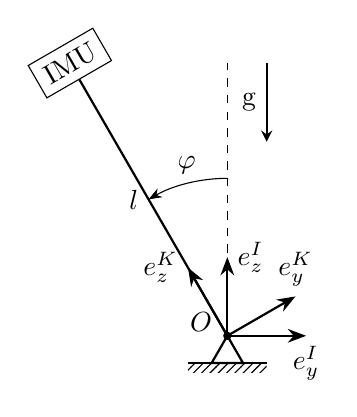
\begin{tikzpicture}[scale=1]
	
	\def\varphiang{-30}
	\def\height{4}
	\def\rArc{0.5*\height}
	
	\def\groundlength{1}
	\def\groundheight_plot{0.12}
	
	\def\supportLength{0.4}
	
	\coordinate (origin) at (0,0);
	\coordinate (originKOS) at ($(origin)$); %-(0.5*\groundlength,0)$);
	\coordinate (IMU) at ($(origin) + ({\height*sin(\varphiang)},{\height*cos(\varphiang)})$);
	
	% Pendulum
	\draw[thick] (origin) -- (IMU) node[midway,left] {$l$};
	
	\draw[dashed](origin) --++ ($({0},{\height*cos(\varphiang)})$);
	
	\draw[-Stealth] ($(origin) + ({0},{\rArc})$) arc(90:90-\varphiang:\rArc) node[midway, above]{$\varphi$};
	
	% IMU
	\node[draw,fill = white, rotate = -\varphiang] at (IMU) {IMU};
	
	% Coordinate System
	\draw[-Stealth,thick] (originKOS) --++ (1,0) node[below]{$e_y^I$};
	\draw[-Stealth,thick] (originKOS) --++ (0,1) node[right]{$e_z^I$};
	
	\draw[-Stealth,thick] (originKOS) --++ ($({cos(\varphiang)},{-sin(\varphiang)})$) node[above]{$e_y^K$};
	\draw[-Stealth,thick] (originKOS) --++ ($({sin(\varphiang)},{cos(\varphiang)})$) node[left]{$e_z^K$};
	
	\fill (origin) circle(1.5pt) node[yshift = -2, xshift = -2, above left]{$O$};
	
	% Ground
	
	
	\coordinate (groundStart) at ($(origin)-(0,{\supportLength*sin(60)})-({0.5*\groundlength},0)$);	
	
	\fill[pattern=north east lines] (groundStart) rectangle ++(\groundlength,-\groundheight_plot);	
	\draw[thick] (groundStart) -- ++(\groundlength,0);	
	
	% Support
	\draw[thick] (origin) --++ ($({\supportLength*cos(60)}, {-\supportLength*sin(60)})$) --++ ($(-\supportLength,0)$) -- (origin);
	
	% Gravity
	\draw[thick,-stealth] ($(origin)+({0.5*\groundlength},{\height*cos(\varphiang)})$) --++(0,-1) node[midway, left]{$\mathrm{g}$};
	
\end{tikzpicture}

	\caption{Pendulum with \acs{IMU} including gravity g.}
	\label{IMG:Setup:Pendulum}
\end{figure}

\input{sec3-analysis}
\input{sec4-experiment}
\input{sec5-outlook}

% Bibliography
\bibliographystyle{IEEEtran}
\bibliography{CCTAScooterIMU}
                                                   

\end{document}
